\chapter{NfM}
\setcounter{section}{0}
%%%%%%%%%%%%%%%%%%%%%%%


\section{Einleitung}
\begin{center}
	\textit{Eine Familie kann das Wunderbarste sein, was man je in seinem Leben erfahren wird.}
\end{center}

Die persönliche Erfahrung zeigt jedoch, wie anspruchsvoll es sein kann, eine Familie zu gründen, sie aufrechtzuerhalten und gemeinsam ein erfülltes Leben zu führen.\\

Diese Strategie - \gls{p_NFM} - zielt darauf ab, dieses Risiko zu minimieren, damit eine Familie tatsächlich das Schönste im Leben sein kann.\\

Die Strategie gliedert sich in drei Teile:
\begin{itemize}
	\item \textit{Objectives}, welche die primären Ziele festhalten, die wir uns für unsere Familie im Bezug zu \gls{p_NFM} setzen und uns Entscheidungshilfen geben sollen.
	\item \textit{\nameref{sec:Erreichung}}, die die Frage klärt, was getan werden kann oder welche Konzepte Anwendung finden, um die \glspl{p_Obj} zu erreichen, und damit eine ausdifferenzierte Entscheidungshilfe darstellen.
	\item und \textit{\nameref{sec:NFMEpilog}}, welche nicht Teil der Strategie ist, jedoch Themen aufgreift, die im Bezug zu \gls{p_NFM} stehen.
\end{itemize}

\begin{figure}[H]
	\centering
	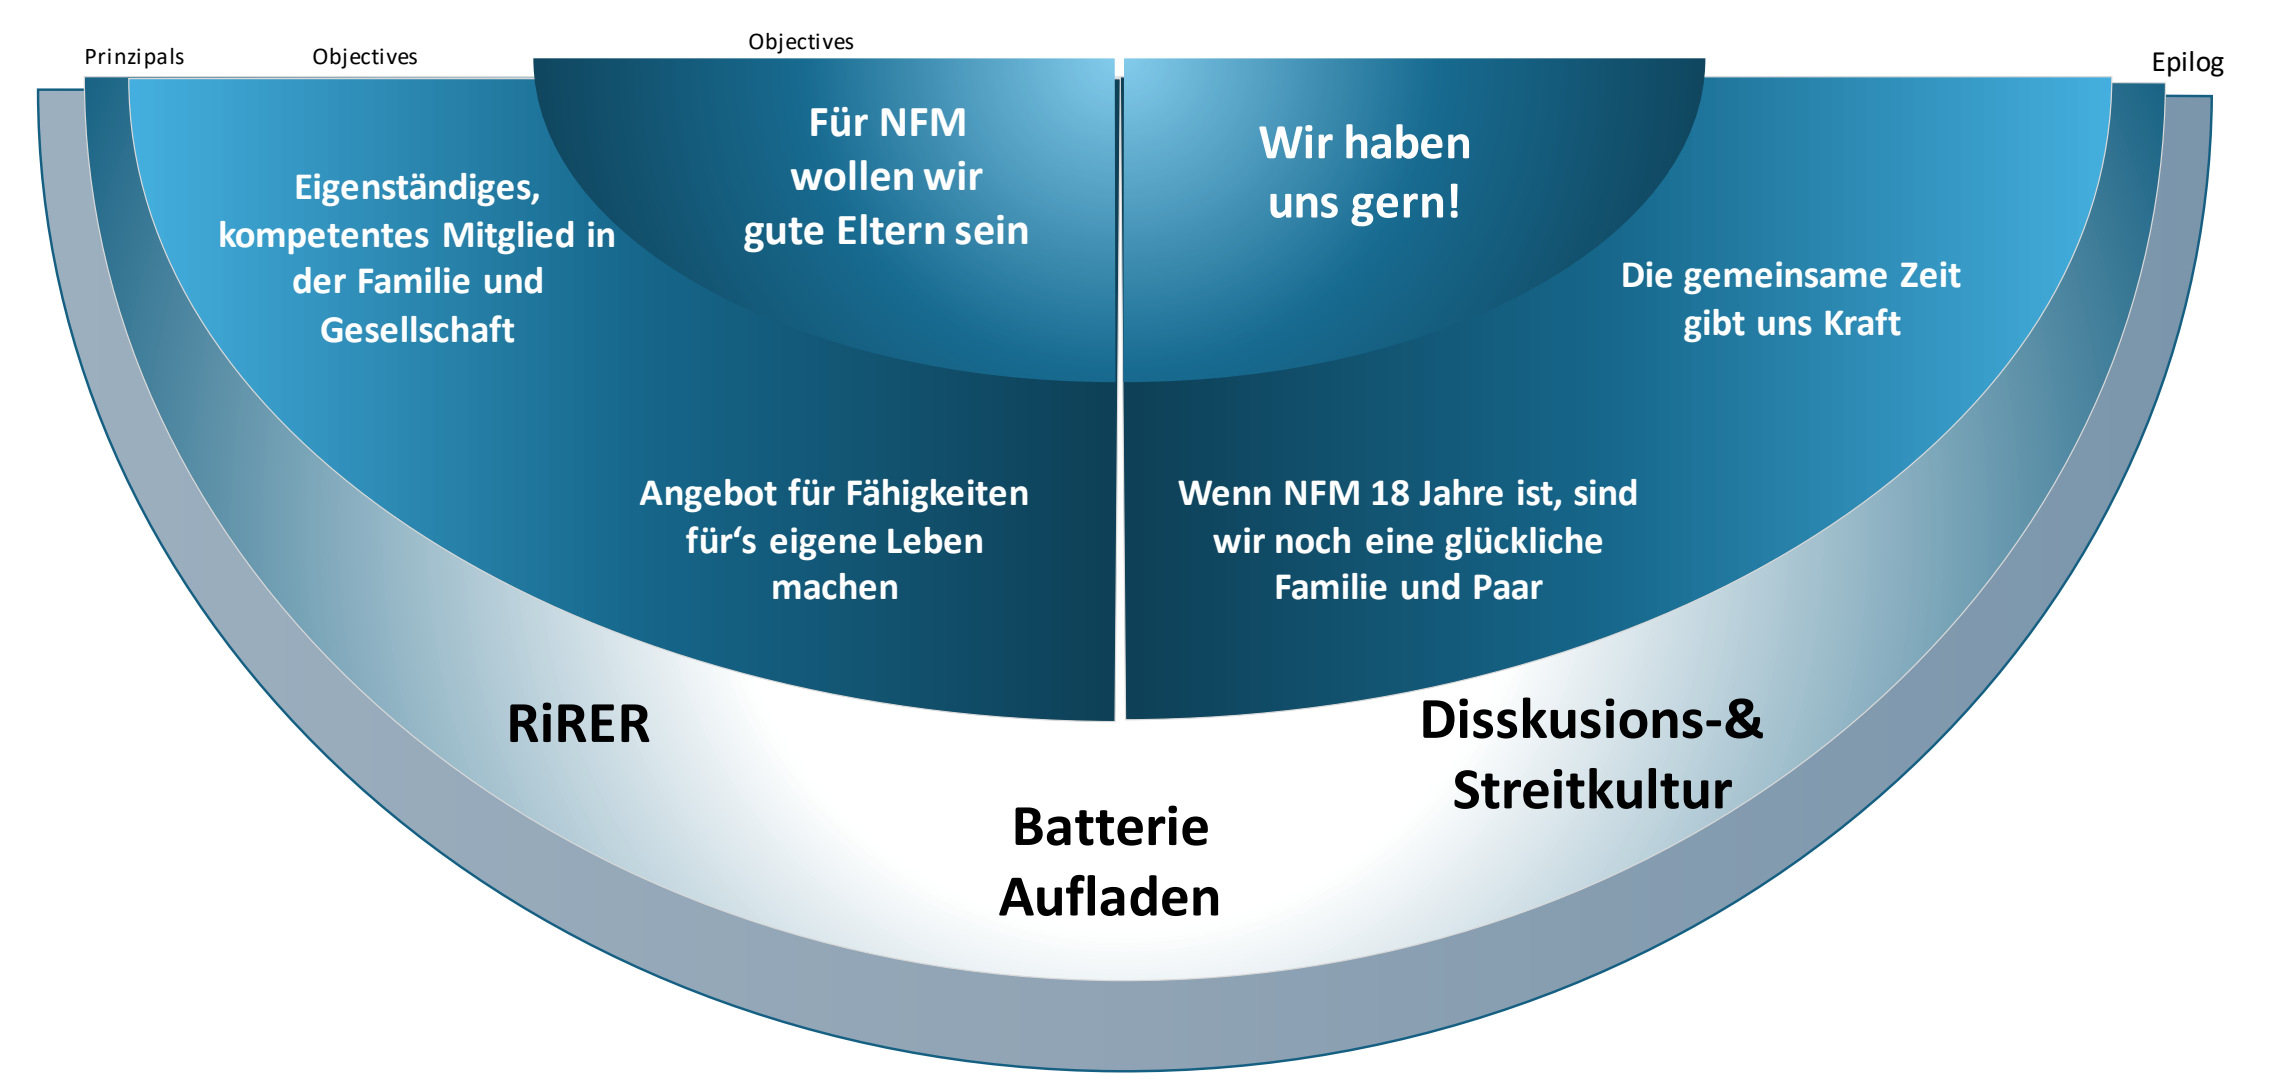
\includegraphics[scale = 0.2]{attachment/chapter_OWN/Scc010.png}
	\caption{Strategie NFM}
\end{figure} 


%Um \gls{p_NFM} eine stabilie Familie zu bieten, auf welcher sie selbst später ihr eigenes Leben fußt, und für uns als Familie 

% One of the greates gift I can ofer them, is that rock, that foundation, to which build there life.
\pagebreak

\section{Objectives} 
%NFM; Strategie Papier Name, Kategorie Name für das NFM

\subsection{Die Vier}

Die folgenden \gls{p_Obj} \footnote{siehe \ref{Appendix_Erlaeuterung_Strategie}} stellen die ersten Ebenen der Strategie da. Die jeweiligen Unterziele stellen ebenso \gls{p_Obj} dar, welche die Zielausrichtung tiefer definieren.

\begin{itemize}
	\item Wir wollen für \gls{p_NFM} gute Eltern sein.
	\begin{itemize}
	\item \gls{p_NFM} ist ein \underline{eigenständiges} $\&$ \underline{kompetentes} Mitglied in der Gesellschaft und der ganzen Familie. \label{NFM_O_1}
	% Alternative Formulierungen
	% 1 Du bist ein eig. und kompet. Mitglied in der Gesellschaft und Familie
	% 2 Wir sind veranwortlich, dass Du ein ...
	% 3 Unsere Elternrolle tragen wir verantwortungsvoll, dass Du ein eig. und kompet. Mitglied in der Gesellschaft und Familie bist.
	\item \gls{p_NFM} bekommt das Angebot, Fähigkeiten für das eigenen Leben zu erlernen. \label{NFM_O_2}
	% Alternative:
	% Strech Goal: Angebot schaffen.
	\end{itemize}
	\item Wir haben uns gern!
	\begin{itemize}
	\item Nach 18 Jahren sind wir noch eine glückliche Familie und Paar.\label{NFM_O_4}
 	\item Die gemeinsame Zeit als Familie gibt uns Kraft. \label{NFM_O_3}
	% Alternative Formulierungen
	% 1 Wir sind eine Familie (Keine Elternrolle), welche uns Kraft und ausnahmslose Sicherheit gibt.
	\end{itemize}
\end{itemize}


Diese \gls{p_Obj} dienen sowohl der Orientierung und Ausrichtung für langfristige Entscheidungen als auch dazu, in wichtigen Momenten bei der Priorisierung zu helfen.\\

Das erste \gls{p_Obj}, \NFMOOne und \NFMOTwo, basiert auf der Überlegung, dass wir als \glspl{p_BFM} eine gesellschaftliche Verantwortung tragen, keine Last für die Gesellschaft zu sein. Im Idealfall ist \gls{p_NFM} eine Bereicherung für Familie und Gesellschaft, oder zumindest keine Belastung.\\

In unserer \gls{p_ER} betrachten wir die Erreichung als unsere Verantwortung. Diese birgt jedoch Risiken, die die Erreichung von \NFMOTwo und \NFMOThree beeinträchtigen können, wie in Abschnitt \ref{sec:Risiko_EKB} beschrieben.\\

Mit \NFMOFour streben wir als \gls{p_FM} kontinuierlich ein erfülltes Leben an und wollen, dass unsere Familie für alle Mitglieder eine Bereicherung ist.\\

Der Unterschied zwischen \NFMOOne und \NFMOFour liegt darin, dass es einen Unterschied zwischen der Integration in die Gesellschaft und der Familie und der Verwirklichung des eigenen Lebens gibt. Das zweite \gls{p_Obj} konzentriert sich darauf, als \gls{p_BFM} die Möglichkeiten aufzuzeigen und gelegentlich \gls{p_NFM} über emotionale Hürden zu begleiten, damit sie selbst entscheiden kann, ob sie diese weiterverfolgt.

\subsection{Analyse} \label{sec:Risiko_EKB}
Der folgende Abschnitt beschäftigt sich damit, welche Risiken in der Familien-Dynamik bestehen. Besonders wird der Schwerpunkt betrachtet, wie erfolgreich die gesetzten \gls{p_Obj} sich realisieren lassen und welche gegenseitigen Abhänigkeiten existieren oder im Wege stehen.\footnote{
	Wie in der näheren Erläuterung von \gls{p_Obj} beschrieben. Die gesetzten Objectives im Bezug zu \gls{p_NFM} haben kein Zeitparameter.
}

\subsubsection{Die initale Hypothese} ist, dass Entscheidungen und Maßnahmen im Zielkonflikt zwischen \NFMOOne, \NFMOTwo und \NFMOThree, \NFMOFour (\textit{Wir haben uns gern}) stehen.\\

Die \gls{p_FM}, in der \gls{p_ER}, sind je nach Situation meist rechtliche, sozial, emotional und wirtschaftliche besser als \gls{p_NFM} positioniert. Dies ist nicht an und für sich kein Problem. Diese Positionierung findet auch außerhalb der Familie statt und dies damit kein alleiniges Merkmal der \gls{p_EKB}.\footnote{
	Im Zeitverlauf wird dies sich auch ändern. Die physische und damit auch kognitive Entwicklung positioniert \gls{p_NFM} besser.
}
Das \gls{p_Obj} \nameref{NFM_O_1} wird jedoch Eingriffe in das Leben von \gls{p_NFM} erfordern. Eine bessere Positionierung in den genannten Kategorien kann jedoch strategisch genutzt werden, die Eingriffe umzusetzen. Weil eine Essens von \nameref{NFM_O_1} ist, dass
\gls{p_NFM} in der Gesellschaft und im Familien-Kontext ihre Kompetenzen integrativ nutzen soll, bedeutet dies eine besser Positionierung von \gls{p_NFM} im Kontext der Familie und Gesellschaft.\\ 

\subsubsection{Conundrum} Die Annahme besteht, dass Eingriffe am besten strategisch realisiert werden\footnote{
	Wichtig: Dies ist unabhängig davon, ob das \gls{p_Obj} damit erreicht wird. Es geht nur um die Veränderung des Verhaltens von \gls{p_NFM}, nicht die interne Überzeugung.
}, wenn die \gls{p_FM} in der \gls{p_ER} besser als \gls{p_NFM} positioniert sind. Gleichzeitig sind die Eingriffe auf eine bessere Positionierung von \gls{p_NFM} ausgelegt.\\

\subsubsection{Risiken}
\begin{itemize}
	\item Ein Risiko ist, dass die Positionierung von \gls{p_NFM} trotz des \gls{p_Obj} nicht erreicht wird, weil der Wunsch besteht, diese Positionierung in der \gls{p_ER} nicht zu verlieren. 
	\item Ein anderes Risiko ist, dass der Eingriff in das eigenen Leben, in dem Fall von \gls{p_NFM}, als ungerecht und störend empfunden wird, welches widerrum \NFMOTwo behindert.
	\item Eine argumentative Beschwichtigung oder Erläuterung mit \gls{p_NFM} kann zu gewissen Zeitpunkten in der physischen Entwicklung nur eingeschränkt möglich sein.
\end{itemize}

Unter Betrachtung dieser Risikoanalyse, wird im nächsten Abschnitt adressiert, wie die \gls{p_Obj} unter der Betrachtung der Risiken erreicht werden können.
% Optional Glossar: Eingriffe

Wie mit diesen Risiken umgegangen werden soll, wird im nächsten Abschnitt behandelt.

\section{Leitende Prinzipien und Konzepte}\label{sec:Erreichung}
% Experimenten Kiste
% Maßnahmen
% Strategische Pillars
% Ideen Pool
% Stratigice Action
% Erreichung
% Guiding Principals
% Guding Concepts
% Leitende Prinzipen/ Mechanismus
\subsection{Übersicht}
Um die drei \glspl{p_Obj} zu erreichen, wird im Folgenden ausgeführt, welche Prinzipien oder Konzepte dazu beitragen.\\

Nicht alle hier beschriebenen Maßnahmen oder Ansätze werden erfolgreich umgesetzt oder erbringen den erhofften Erfolg. Der Zweck dieses Abschnitts ist jedoch, sich im Vorfeld darüber klar zu werden, wie die genaue Erreichung der \gls{p_Obj} angegangen werden kann, wie diese mit anderen Aktionen im Einklang oder nicht im Einklang steht und welche Annahmen der Umsetzung bestimmter Aktionen oder Konzepte zugrunde liegen.\\

Hierbei handelt es sich um bisherige Ideen, die nun in den kohärenten Rahmen von \gls{p_NFM} gebracht werden. Nicht alle bisherigen Ideen werden für den ersten Entwurf hier integriert werden, weil sie entweder nicht weit genug durchdacht sind, nicht mit den Zielsetzungen vereinbar sind oder weil die Zeit nicht ausreicht, um sich mit allen vorherigen Gedanken intensiv auseinanderzusetzen. Themen, die sich nicht mit \gls{p_NFM} vereinigen lassen, aber dennoch sinnvoll sind, werden in Abschnitt \ref{sec:NFMEpilog} ausgeführt.\\

Ebenso werden einige dieser Maßnahmen und Konzepte sich im Zeitverlauf entwickeln, weil neue Ideen entstanden sind, wie ein erfolgreicherer Ansatz gestaltet werden kann, oder neue Erkenntnisse aus dem Ausprobieren hervorgegangen sind. Ein kontinuierliches schriftliches Update dieser ist vorerst nicht vorgesehen.


\subsection{Reduzierung der Relevanz der Elternrolle - \gls{p_RiRER}}

Ein Prinzip, das besonders in den ersten 18 Jahren der \gls{p_EKB} Anwendung finden wird, ist \gls{p_RiRER}.\\
% Was es mit dem Risiko zu tun hat, wird später erläutert.

Um dies zu erreichen, werden drei Kategorien betrachtet:\footnote{
	Hierbei sind Entscheidungen gemeint, welche direkt oder indirekt für \gls{p_NFM} getroffen werden; Besonders finanzielle und soziale Netzwerk-Ressourcen besitzt \gls{p_NFM} zum Start noch nicht; Nicht alle Unterfangen kann \gls{p_NFM} selbstständig angehen. Meist bedarf es Fähigkeiten, ein gewisses Unterfangen durchzuführen. Selbst wenn das Unterfangen selbst von \gls{p_NFM} durchgeführt werden kann, die anderen Fähigkeiten nicht.
} 
\begin{itemize}
	\item Entscheidungen,
	\item Ressourcen
	\item und Betreuung
\end{itemize}

\subsubsection{Transit}
Bei diesen Kategorien soll ein Transit erfolgen, der die \gls{p_RiRER} reduziert und somit zu \nameref{NFM_O_1} beiträgt. Der Verlauf wird nicht linear erfolgen, jedoch soll durch die kontinuierliche Übergabe von Verantwortung, Vermittlung von Kompetenzen und Reduktion von beeinflussenden Entscheidungen in \gls{p_NFM}s Leben sichergestellt werden, dass \nameref{NFM_O_1} kontinuierlich überprüft werden kann, um den Erfolg von \gls{p_RiRER} zu bewerten. 

Wir antizipieren, dass an gewissen Abschnitten im Leben von \gls{p_NFM} die Relevanz für die \gls{p_ER} wieder ansteigen wird, um entweder gesellschaftliche Hürden zu überwinden oder physische Entwicklungsschritte zu bewältigen, die sich negativ auf \nameref{NFM_O_1} oder \NFMOTwo auswirken.

\begin{figure}[H]
	\centering
	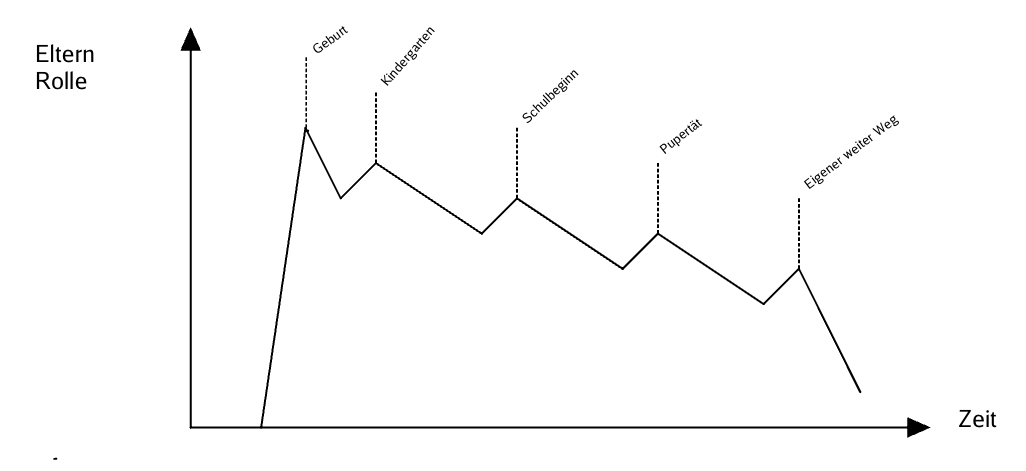
\includegraphics[scale = 0.3]{attachment/chapter_OWN/Scc005.png}
	\caption{Versinnbildlichung der Relevanz der \gls{p_ER} im Zeitverlauf}
\end{figure} 

\subsubsection{Raum zur Debatte} 
Wie weit der Transit vollzogen ist und wie weit die drei \gls{p_Obj} vorangeschritten sind, wird sich nicht eindeutig bestimmen lassen oder von allen gleich aufgefasst werden. Um dies als Familie permanent auszuloten, benötigt es Raum zur Debatte. Vor allem für \gls{p_NFM} sehen wir es als wichtig an, dass dieser Raum gegeben wird, um
\begin{itemize}
	\item unsere Annahmen, Schlussfolgerungen und angeleiteten Maßnahmen herauszufordern, 
	\item eigene Themen einzubringen
	\item und gemeinschaftlich über den aktuellen Status zu reflektieren.
\end{itemize}

Dies steht ebenso in Abhängigkeit unter \ref{subsec_LeitendePrinzipien_Diskussionskultur}.

\subsubsection{Schwerpunkt Maßnahmen}

\begin{figure}[H]
	\centering
	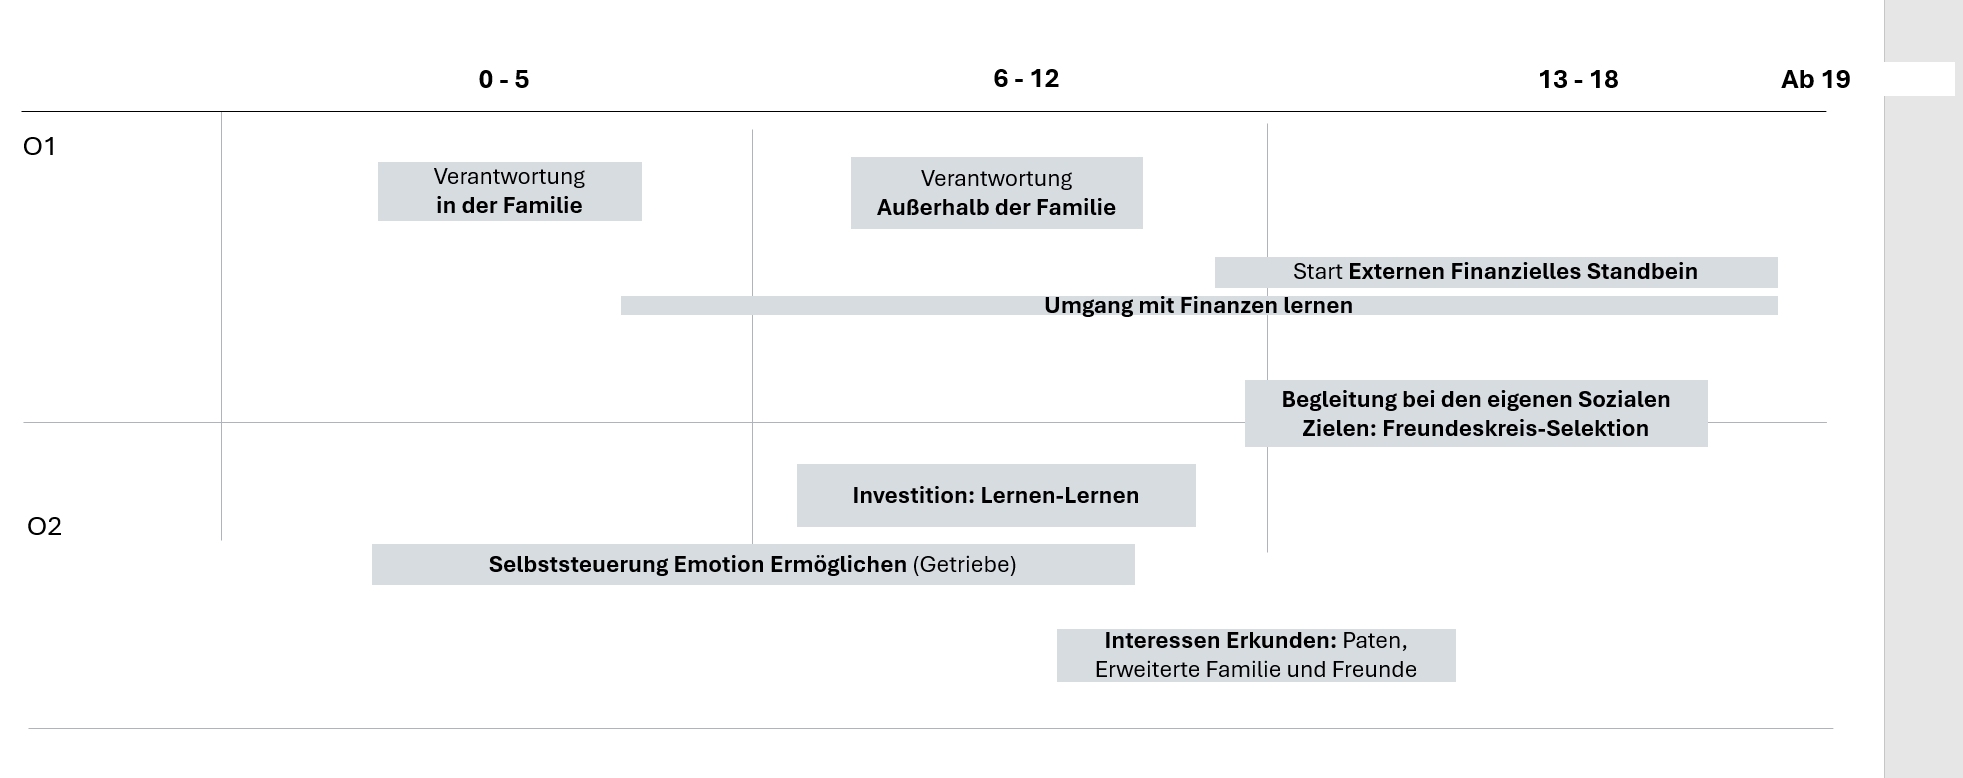
\includegraphics[scale = 0.3]{attachment/chapter_OWN/Scc008.png}
	\caption{Schwerpunkt Maßnahmen im Zeitverlauf}
\end{figure}

\paragraph{Umgang mit Geld}
Mit Abnahme der \gls{p_RiRER} geht einher, dass \gls{p_NFM} mehr Verantwortung in der Familie und Gesellschaft bekommt.\\

Der Umgang mit Geld ist ein Standbein, welcher dabei hilft, eine Reduktion bei den Ressourcen zu kompensieren. Ein möglicher Ansatz ist, dass \gls{p_NFM} ein eigenes gemeinsames Konto bekommt. Auf diesen Zahlen wird für es eingezahlt, alle Ausgaben für \gls{p_NFM} werden darüber getätigt.

Ab einen gewissen Zeitpunkt, bekommt \gls{p_NFM} selbst Zugang zu diesem Konto, von welchem es die eigen Sachen bezahlen kann. Die Fähigkeit, welche \gls{p_NFM} dabei erlangen soll, ist mit limitieren Ressourcen umzugehen. Anderes, als wenn die \gls{p_NFM} die \gls{p_FM} fragt, und diese es zahlen.\footnote{
	Hierbei gibt es keine limitierte Ressource, weil die \gls{p_FM} immer gefragt werden kann.
} Die \gls{p_FM} helfen vor allem im ersten Prozess. \footnote{
	Zusätzlich kann hierbei Plus und Minus schon gelernt werden.
}

\paragraph{Freundeskreis Auswahl}

Während der Pubertät ist die Auswahl des Freundeskreises entscheidend.\\

Bei der Auswahl der Freundesgruppe ist darauf zu achten, welcher symbolische Akt der Anerkennung (Status) erforderlich ist, um den jeweiligen Status in der Gruppe aufrechtzuerhalten.\\

Es ist mit hoher Wahrscheinlichkeit zu erwarten, dass ein solcher Akt vollzogen werden muss oder sogar gewollt ist.\\

Die Kontrollgröße bleibt die Auswahl der Gruppe, anhand derer die Mitglieder nach Anerkennungssymbolen ausgewählt werden. Nicht immer wird es möglich sein, frei eine Freundesgruppe auszuwählen. Jedoch sollte bei der langfristigen Wahl des Freundeskreises darauf geachtet werden, ob Anerkennungssymbole erbracht werden müssen, die möglicherweise langfristig negative Auswirkungen auf das eigene Leben oder das Leben anderer haben, z.B.: einen Raub zu begehen, um Anerkennung zu erhalten. Solche Mutproben werden in der ein oder anderen Form von der Gruppe verlangt.\\

Für \gls{p_NFM} sollte daher ein Kriterium sein, ob es sich einer Gruppe anschließt, welche Anerkennungssymbole in der Gruppe erbracht werden müssen und dann mit den eigenen Wertvorstellungen abgeglichen werden. Wenn dies im Vorfeld nicht erfolgt, besteht ein höheres Risiko, dass Anerkennungssymbole durchgeführt werden, obwohl sie einem oder anderen schaden könnten. Denn wenn man einmal in der Gruppe ist, ist es schwieriger, sich dem Statusspiel zu entziehen, da dies eine Veränderung erfordern würde.\\

Positive Kriterien könnten Mut im geistigen oder körperlichen Wettbewerbsaspekt sein, zum Beispiel besonders lustig zu sein oder bei einer sportlichen Aktivität besonders mutig zu sein (Canyoning 15 Meter Sprung).\\

Diese Anerkennungssymbole müssen daher nicht notwendigerweise erbracht werden. Es kann jedoch so sein, dass sie als Teil des Statusspiels verstanden werden. Was für eine Gruppe jedoch wichtig ist, ist, dass gewisse Eigenschaften offenbart werden, die die Gruppe definieren. Zum Beispiel ist es erwünscht, besonders gesellig zu sein und gut im Umgang mit anderen. Vielleicht ist es nicht erforderlich, immer gut drauf zu sein, aber gut musizieren zu können.\\

Die Auswahl der Gruppe ist daher ein ganz besonderer Schritt und prägt einen stark, da bestimmte Aspekte verstärkt oder unterdrückt werden können.

\paragraph{Investition: Lernen-Lernen}

Für mich selbst bedeutet dies, dass ich regelmäßig Zeit einplane, um mit \gls{p_NFM} zu lernen und die Lernergebnisse zu bewerten und Feedback zu geben. Diese Maßnahme trägt sowohl zu \NFMOOne als auch zu \NFMOThree bei. Dies geschieht, weil zum einen ein Angebot gemacht wird, diese Fähigkeit zu erlernen und Zeit zu investieren, und zum anderen, um langfristig unabhängig für das weitere Leben zu sein.

Zwei Mantras/Fragen sollen dabei unterstützen:
\begin{itemize}
	\item Die letzten 5 Prozent sind für die Qualität der Arbeit entscheidend.
	\item Die ernst gemeinte Frage wird gestellt: Ist dies das beste Ergebnis, das du erreichen kannst?
\end{itemize}

\paragraph{Verantwortung innerhalb und außerhalb der Familie}

Mit jeder Stufe der Übernahme von Verantwortung geht auch eine Ebene der Gleichheit in der Familienhierarchie einher. Wer Verantwortung trägt, kann auch mitbestimmen.

Von 0 bis 6 Jahren sind wir die Hauptbezugspersonen. Wir werden versuchen, dies auszugleichen, indem wir Familie und Freunde frühzeitig in die Erziehung integrieren.

\subsection{Batterien aufladen}

Um den "Akku" jedes \gls{p_FM} aufzuladen, benötigt es Zeit, in der jeder frei von Verantwortung ist oder Dinge tun kann, die die Energiereserven wieder auffüllen.

Die Zielsetzung hier ist recht einfach. Die \gls{p_BFM} haben die Verantwortung und Pflicht, auf sich selbst zu achten, damit sie die Kraft und Geduld für die oberen Zielsetzungen haben und kognitiv nicht eingeschränkt sind.

\subsection{Diskussions- und Streitkultur gemeinsam leben}\label{subsec_LeitendePrinzipien_Diskussionskultur}

Es ist wichtig, dass wir uns als Paar und Familie angemessen Zeit für Diskussion und Streit nehmen!\\

Eine erste Diskussions- und Streitkultur hat sich bei uns als Paar bereits entwickelt. Die Anpassung daran findet kontinuierlich statt. Allerdings haben wir festgestellt, dass sich Zeit für Diskussionen und Streit nicht planen lässt. Zum Beispiel können wir nicht regelmäßig Termine festlegen, um Themen zu debattieren, die uns beschäftigen. In unserer Diskussions- und Streitkultur geben wir uns zeitnah Rückmeldungen darüber, welche Themen uns beschäftigen und in anderen Bereichen unseres Lebens beeinträchtigen.\\

Im Hinblick auf \gls{p_NFM} erkennen wir das Risiko, dass zunehmende Alltagsthemen und eine größere organisatorische Abhängigkeit von Familie und Freunden den Eindruck vermitteln können, dass weniger Zeit für Diskussionen und Streit möglich ist. Daher folgern wir, dass wenn Themen auftauchen, die eine Diskussion oder einen Streit erfordern, wir sie nicht als \textit{on-Top} betrachten sollten, sondern als \textit{Investition} für die Erreichung der \gls{p_Obj}, insbesondere für \NFMOOne und \NFMOThree. Ebenso ist es für \gls{p_RiRER} entscheidend, dass diese Fähigkeit ausreichend vorhanden ist, um gemeinsam die einzelnen Phasen von \gls{p_RiRER} zu durchlaufen.